\documentclass[a4paper,12pt]{article}

%%%%%%%%%%%%%%%%%%%%%%%%%%%%%%%%%%%%%%%%%%%%%%%%
% Packages
%%%%%%%%%%%%%%%%%%%%%%%%%%%%%%%%%%%%%%%%%%%%%%%%

\usepackage[right=2.5cm, left=2.5cm, top=2.5cm, bottom=2.5cm]{geometry} 
\usepackage[portuguese]{babel}
\usepackage[T1]{fontenc}
\usepackage[utf8]{inputenc}
\usepackage{url}
\usepackage{hyperref}
\Urlmuskip=0mu  plus 10mu

% no indentation
%\usepackage{setspace}
%\setlength{\parindent}{0in}

\usepackage{graphicx} 
\usepackage{float}
\usepackage{xcolor}

\usepackage{mathtools}
\usepackage{amssymb, amsthm}

% headers
\usepackage{fancyhdr}

%%%%%%%%%%%%%%%%%%%%%%%%%%%%%%%%%%%%%%%%%%%%%%%%
% Proper definitions
%%%%%%%%%%%%%%%%%%%%%%%%%%%%%%%%%%%%%%%%%%%%%%%%
\newcommand{\R}{\mathbb{R}}

\newtheoremstyle{exer}{}{}{\color{blue}}{}{\color{blue}\bfseries}{}{ }{}
\theoremstyle{exer}
\newtheorem{exercise}{Exercício}

\theoremstyle{definition}
\newtheorem{solution}{Solução}

\theoremstyle{plain}
\newtheorem{remark}{Observação}



%%%%%%%%%%%%%%%%%%%%%%%%%%%%%%%%%%%%%%%%%%%%%%%%
% Header (and Footer)
%%%%%%%%%%%%%%%%%%%%%%%%%%%%%%%%%%%%%%%%%%%%%%%%

\pagestyle{fancy} 
\fancyhf{}

\lhead{\footnotesize CS: Lista 2}
\rhead{\footnotesize Prof. Asla e Mon. Lucas} 
\cfoot{\footnotesize \thepage} 


\begin{document}

%%%%%%%%%%%%%%%%%%%%%%%%%%%%%%%%%%%%%%%%%%%%%%%%
% Title section of the document
%%%%%%%%%%%%%%%%%%%%%%%%%%%%%%%%%%%%%%%%%%%%%%%%

\thispagestyle{empty} 

\begin{tabular*}{0.95\textwidth}{l @{\extracolsep{\fill}} r} 
    {\large \bf Curvas e Superfícies 2022.1} &  \\
    Escola de Matemática Aplicada, Fundação Getulio Vargas &  \\
    Professora Asla Medeiros e Sá &  \\ 
    Monitor Lucas Machado Moschen & Entrega 07/03/2021\\
    \hline \\
\end{tabular*} 
\vspace*{0.3cm} 

\begin{center}
	{\Large \bf Lista 2} 
	\vspace{2mm}
	%{\bf Lucas Machado Moschen}	
\end{center}  
\vspace{0.4cm}

\begin{exercise}
    Desenhe em ambiente computacional, utilizando sistemas de computação
    simbólica, incluindo a animação do vetor tangente percorrendo as seguintes
    parametrizações da parábola $\alpha(t) = (t, t^2)$ e $\gamma(t) = (t^3,
    t^6)$. Mostre que $\alpha$ é curva regular e $\gamma$ não é regular. Qual
    seria a função naturalmente candidata a ser uma reparametrização entre as
    duas parametrizações? Porque falha?
\end{exercise}

\begin{solution}
    Confira a imagem produzida no Geogebra na Figura \ref{fig1}
    \begin{figure}[hb]
        \centering
        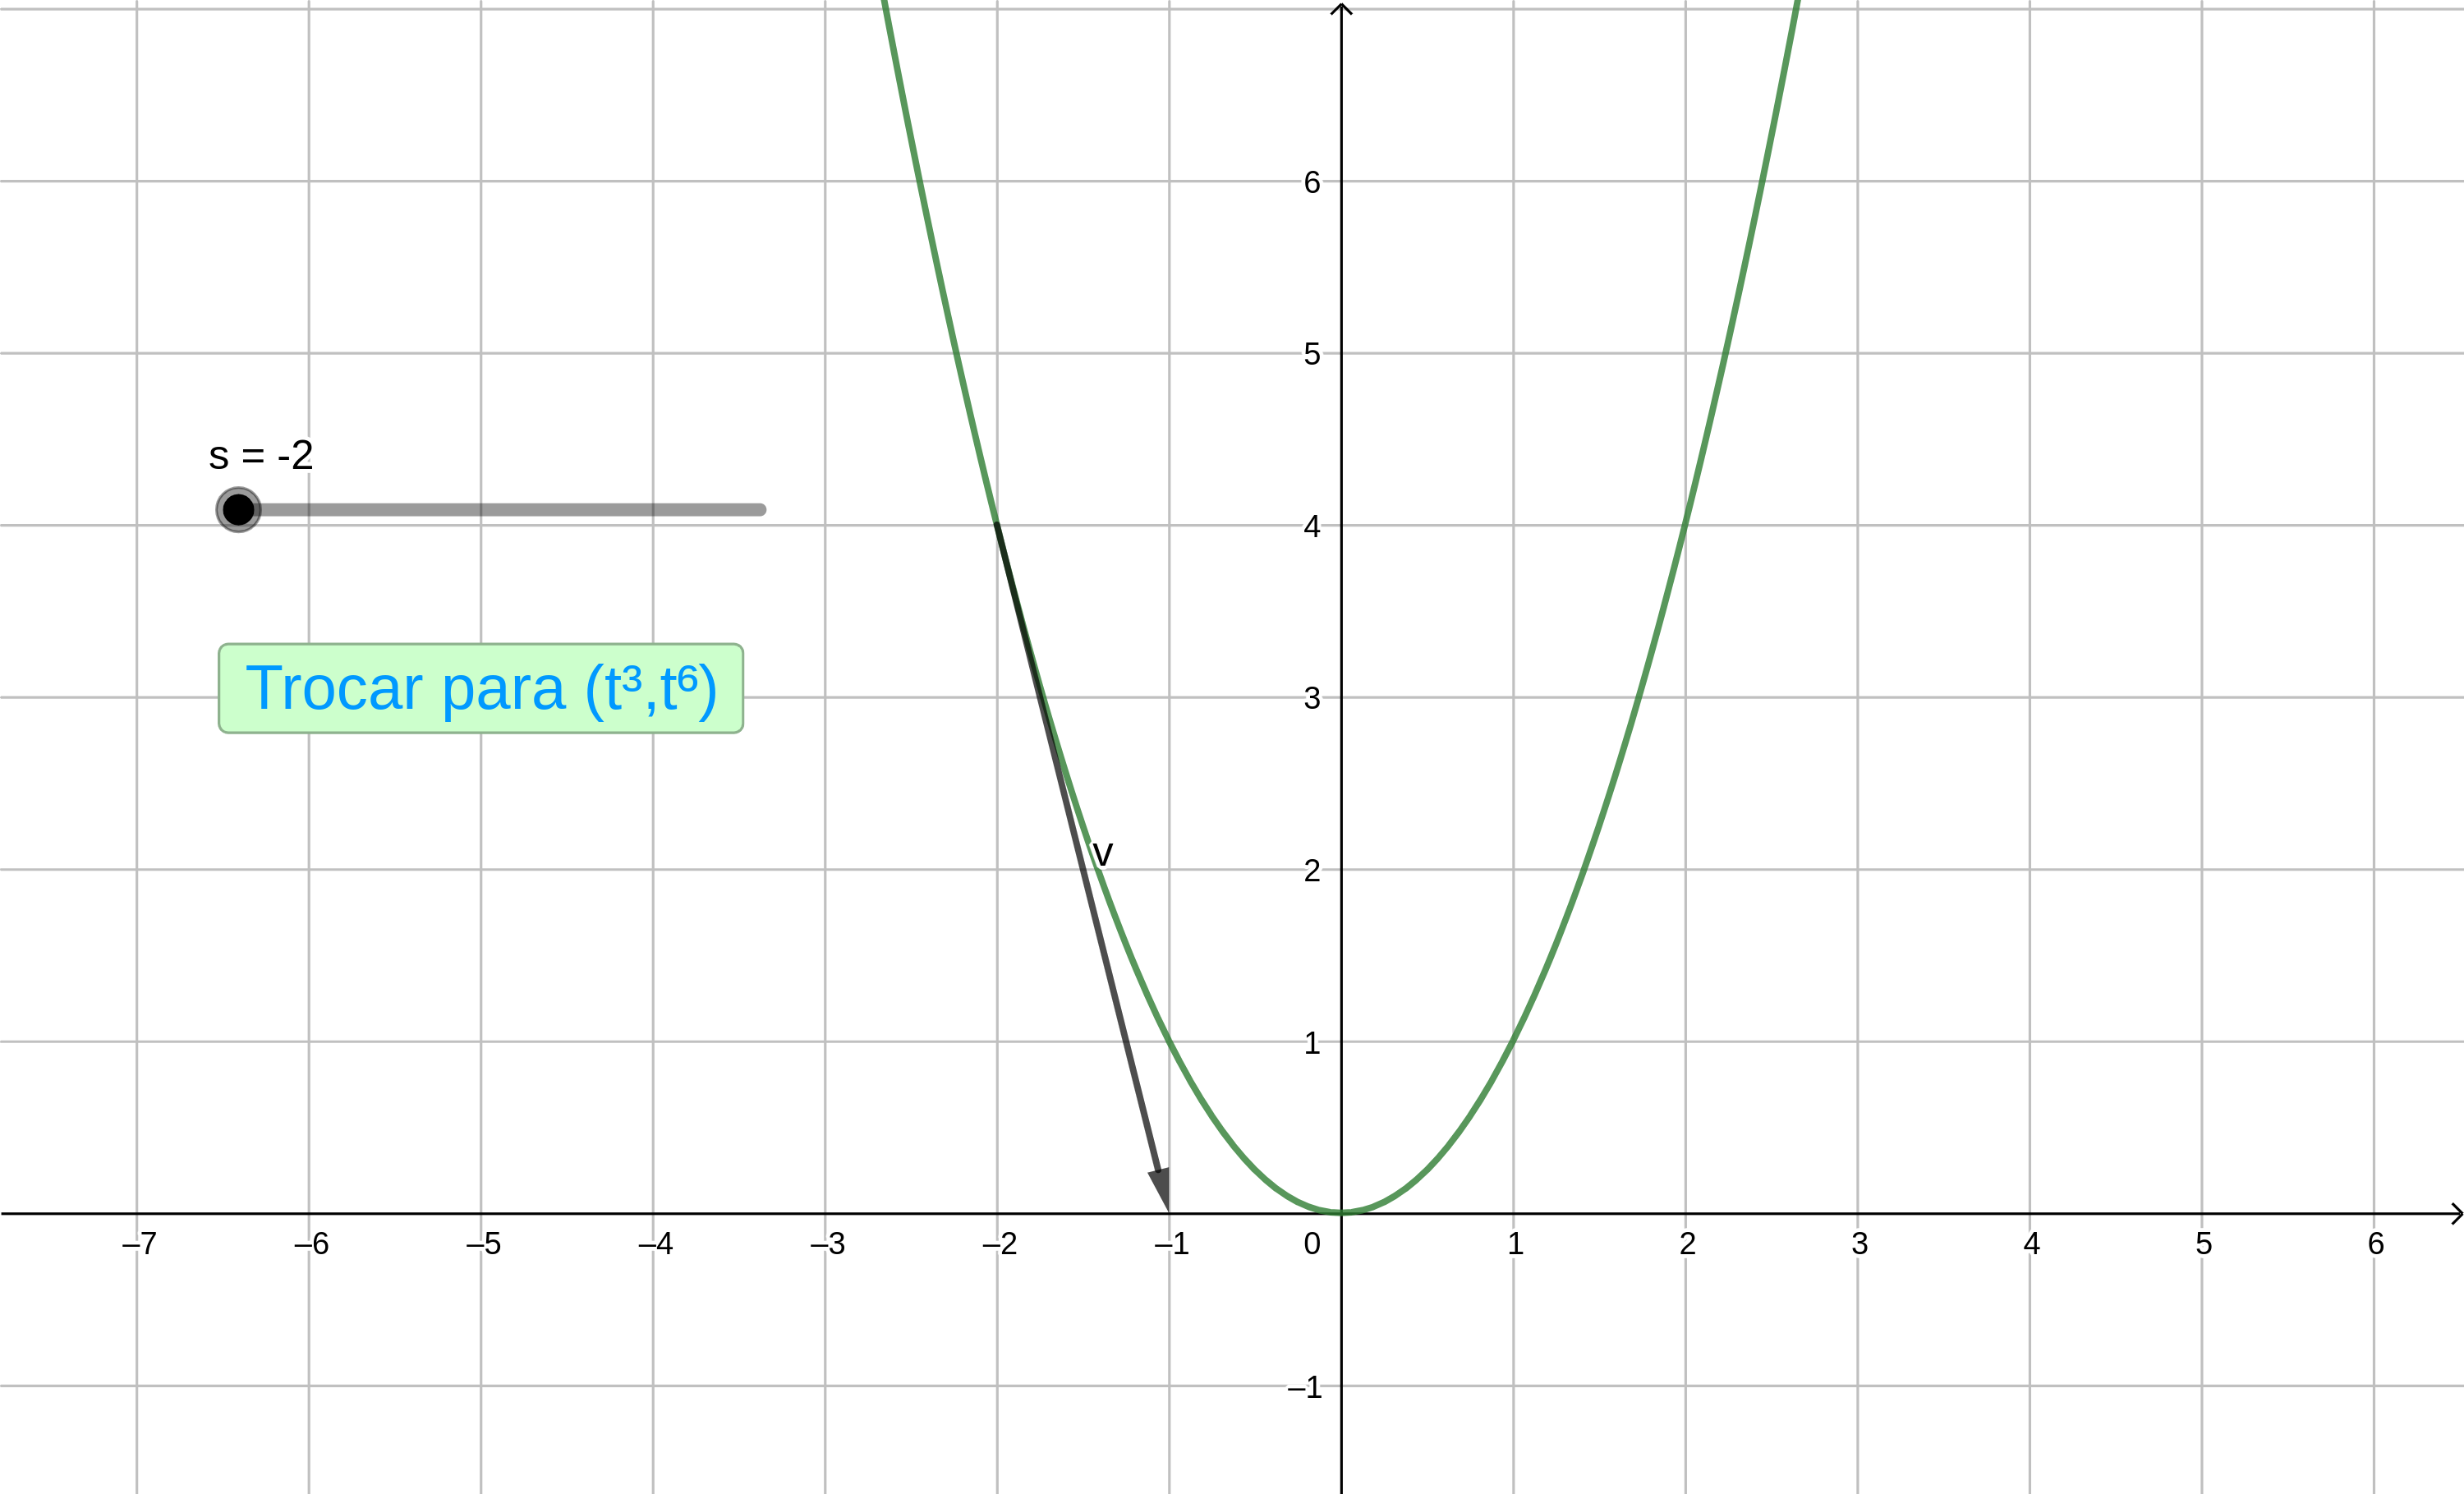
\includegraphics[width=\textwidth]{images/exe1.png}
        \caption{Exercício 1}
        \label{fig1}
    \end{figure}
    Você pode conferir no Github
    também\footnote{\url{https://github.com/lucasmoschen/ta-sessions/blob/master/Curves_Surfaces/lists/list2/exercicio1.ggb}}.
    
    Observe que $||\alpha'(t)|| = ||(1,2t)|| > 0$, pois o vetor $(0,2t)$ é não
    nulo para todo $t \in \R$. Portanto $\alpha$ é uma curva regular. Todavia
    $||\gamma'(t)|| = ||(3t^2, 6t^5)|| = 0$ se, e somente se, $t = 0$. Na
    animação, podemos observar claramente a quando o vetor é nulo e
    "desaparece". Logo $\gamma$ é não regular. A fim de que elas fossem uma
    reparametrização da outra, a função $h:\R \to \R$ definida como $h(x) =
    x^3$ é uma candidata natural. Pelo lema que provarei a seguir, $h$ não
    pode ser um difeomorfismo pois $h'(0) = 0$ e por isso a reparametrização falha. 

    {\bf Afirmação:} Se $h$ é um difeomorfismo, não pode ter derivada nula em
    ponto algum. Seja $g = h^{-1}$, de forma
    que $\tilde{t} = g(t)$. Assim $h(g(t)) = t$ e, portanto, pela regra da
    cadeia, 
    $$
    \frac{dh}{d \tilde{t}} \frac{dg}{dt} = 1
    $$
    Em particular, $\frac{dh}{d\tilde{t}} \neq 0, \forall t$. 
\end{solution}

\begin{exercise}
    Mostre que as curvas regulares $\alpha(t) = (t, e^t), t \in \R $ e
    $\beta(s) = (\log(s), s), s \in (0,\infty)$ têm o mesmo traço.
\end{exercise}

\begin{solution}
    Temos que provar que os conjuntos imagem $\alpha(\R)$ e
    $\beta((0,+\infty))$ são iguais. Para isso, vamos provamos a dupla
    inclusão. 

    \begin{enumerate}
        \item Tome $(x,y) \in \alpha(\R)$. Portanto, existe $t$, tal que $x =
        t$ e $y = e^t$. Tome $s = e^t > 0$. Então $\log(s) = t = x$, e nesse
        caso, $(x,y) = (\log(s), s)$, o que implica que $(x,y) \in
        \beta((0,+\infty))$ e $\alpha(\R) \subseteq \beta((0,\infty))$. 
        
        \item Tome $(x,y) \in \beta((0,\infty))$. Assim existe $s$ de forma
        que $x = \log(s)$ e $y = s$. Tome $t = \log(s)$ e teremos que $x = t$
        e $y = e^t$, portanto $\beta((0,+\infty)) \subseteq \alpha(\R)$
    \end{enumerate}
    Concluímos que $\alpha(\R) = \beta((0,+\infty))$. Outra possível solução
    seria provar que essas curvas são reparametrização uma da outra. 
\end{solution}

\begin{exercise}
    Calcule o comprimento de arco das seguintes curvas:
    \begin{enumerate}
        \item $\alpha(t) = (3\cosh(2t), 3\sinh(2t),6t), t \in [0, \pi]$
        \item Catenária: $\gamma(t) = (t,\cosh(t))$ a partir do ponto $(0,1)$.
    \end{enumerate}
\end{exercise}

\begin{solution}
    Aqui basta lembrar a fórmula de comprimento de arco 
    $$
    L_a^b(\alpha) = \int_a^b ||\alpha '(t)||dt
    $$
    Por exemplo, na primeira, tomando $a = 0$, temos 
    $$
    L_0^t(\alpha) = \int_0^t 6||(\sinh(2s), \cosh(2s), 1)||ds = \int_0^t 6(\sinh^2(2s) + \cosh^2(2s) + 1)^{1/2}ds
    $$
    Note que $\cosh^2(x) - \sinh^2(x) = 1$ e que $\cosh(x) > 0$, e então, 
    $$
    L_0^t(\alpha) = 6\sqrt{2}\int_0^t \cosh(2s)ds = 3\sqrt{2}\sinh(2t)
    $$
    Em particular $L_0^{\pi}(\alpha) = 3\sqrt{2}\sinh(2\pi)$. Para fazer o
    segundo exercício, basta calcular $L_0^t(\gamma)$ usando o mesmo
    princípio, mas uso o ferramental do GeoGebra e, por isso, confira no
    GitHub o
    arquivo\footnote{\url{https://github.com/lucasmoschen/ta-sessions/blob/master/Curves_Surfaces/lists/list2/exercicio3.ggb}}.
    \begin{figure}[ht]
        \centering
        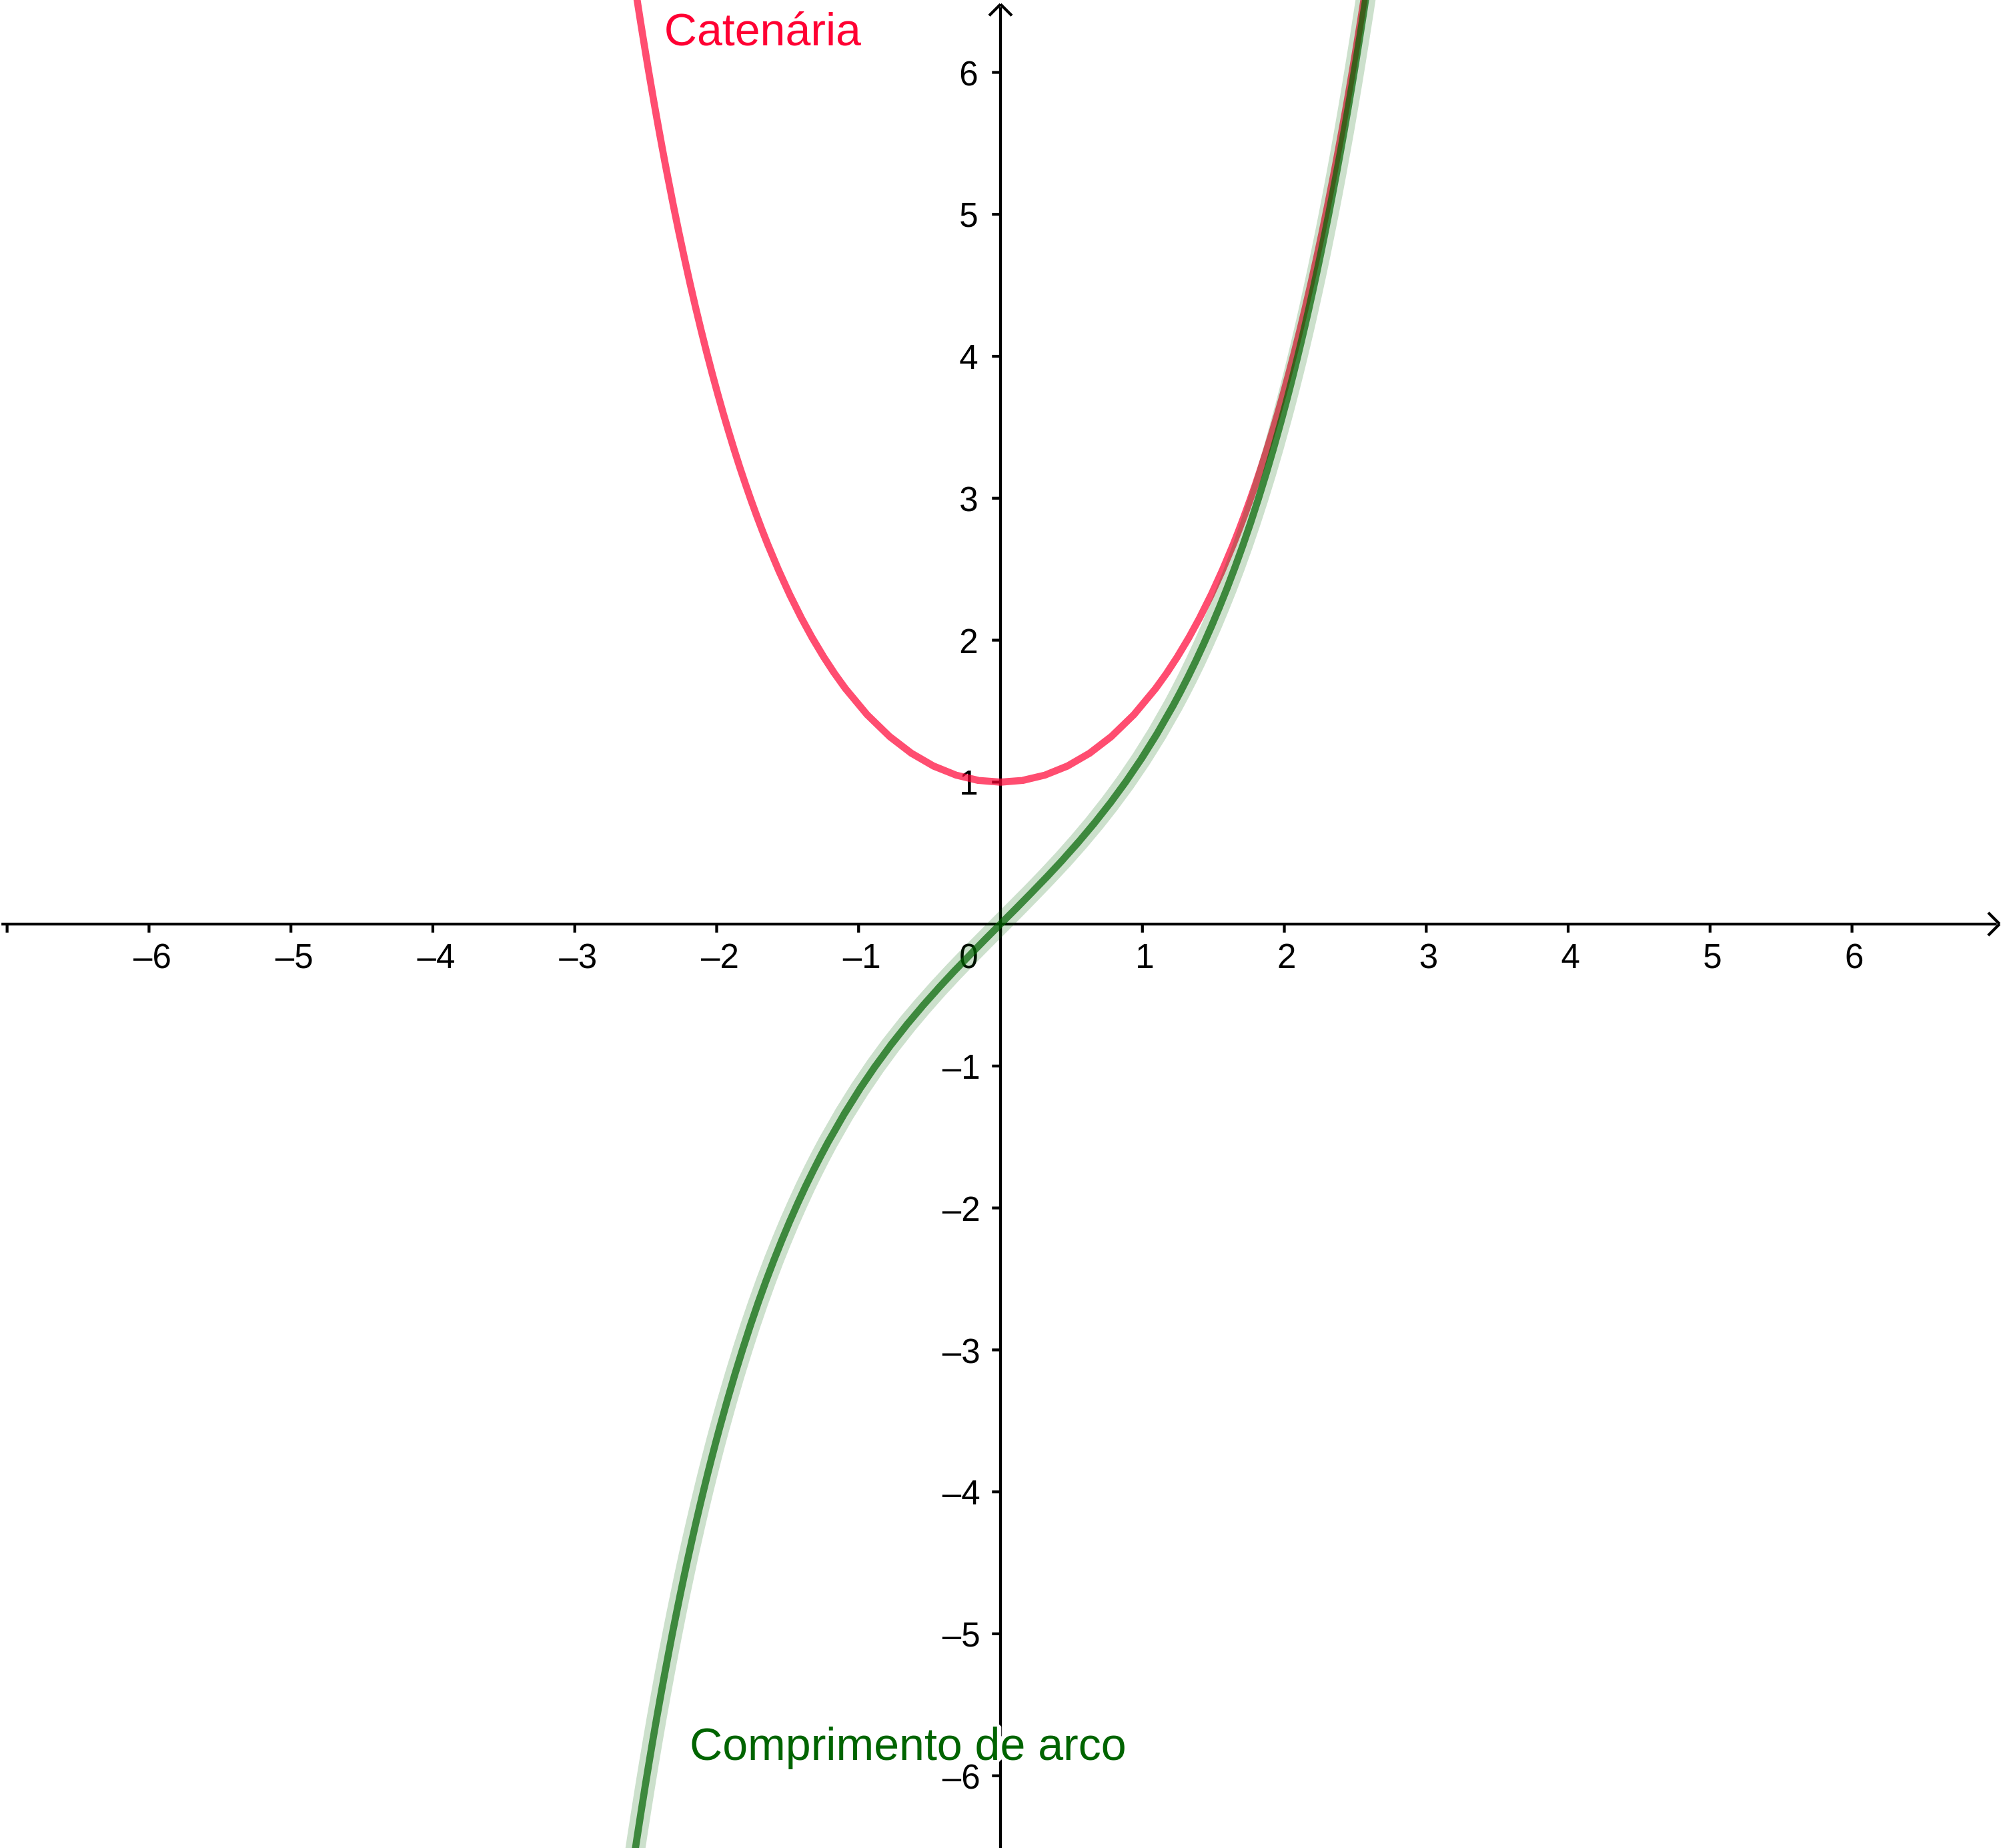
\includegraphics[width=0.7\textwidth]{images/exe3.png}
        \caption{Exercício 3}
        \label{fig2}
    \end{figure}
\end{solution}

\begin{exercise}
    Mudanças de parâmetro:
    \begin{enumerate}
        \item  Demonstrar que $s(\theta) = \dfrac{\theta^2}{\theta^2 + 1}$ é uma mudança de parâmetro diferenciável que
        transforma o intervalo $(0,\infty)$ no intervalo $(0, 1)$.
        \item Mostrar que a função $\gamma : (-1, 1) \to (-\infty, +\infty)$
        definida por $\gamma(t) := \tan(\pi t/2)$ é uma mudança de parâmetro.
        \item Provar que qualquer curva pode ser reparametrizada de forma tal que o domínio
        da reparametrização seja um intervalo de extremos 0 e 1.
    \end{enumerate}
\end{exercise}

\begin{solution}
    Exercícios como esse são mais extensos e, por esse motivo, não demonstrei
    usando latex. Para mostrar que cada uma dessas aplicações é uma mudança de
    parâmetro dever ser mostrada a bijetividade, continuidade e
    diferenciabilidade dela e de sua inversa. Algumas indicações foram feitas
    no papel. Não conferi muito as contas, então qualquer dúvida, só avisar.
    \begin{figure}
        \centering
        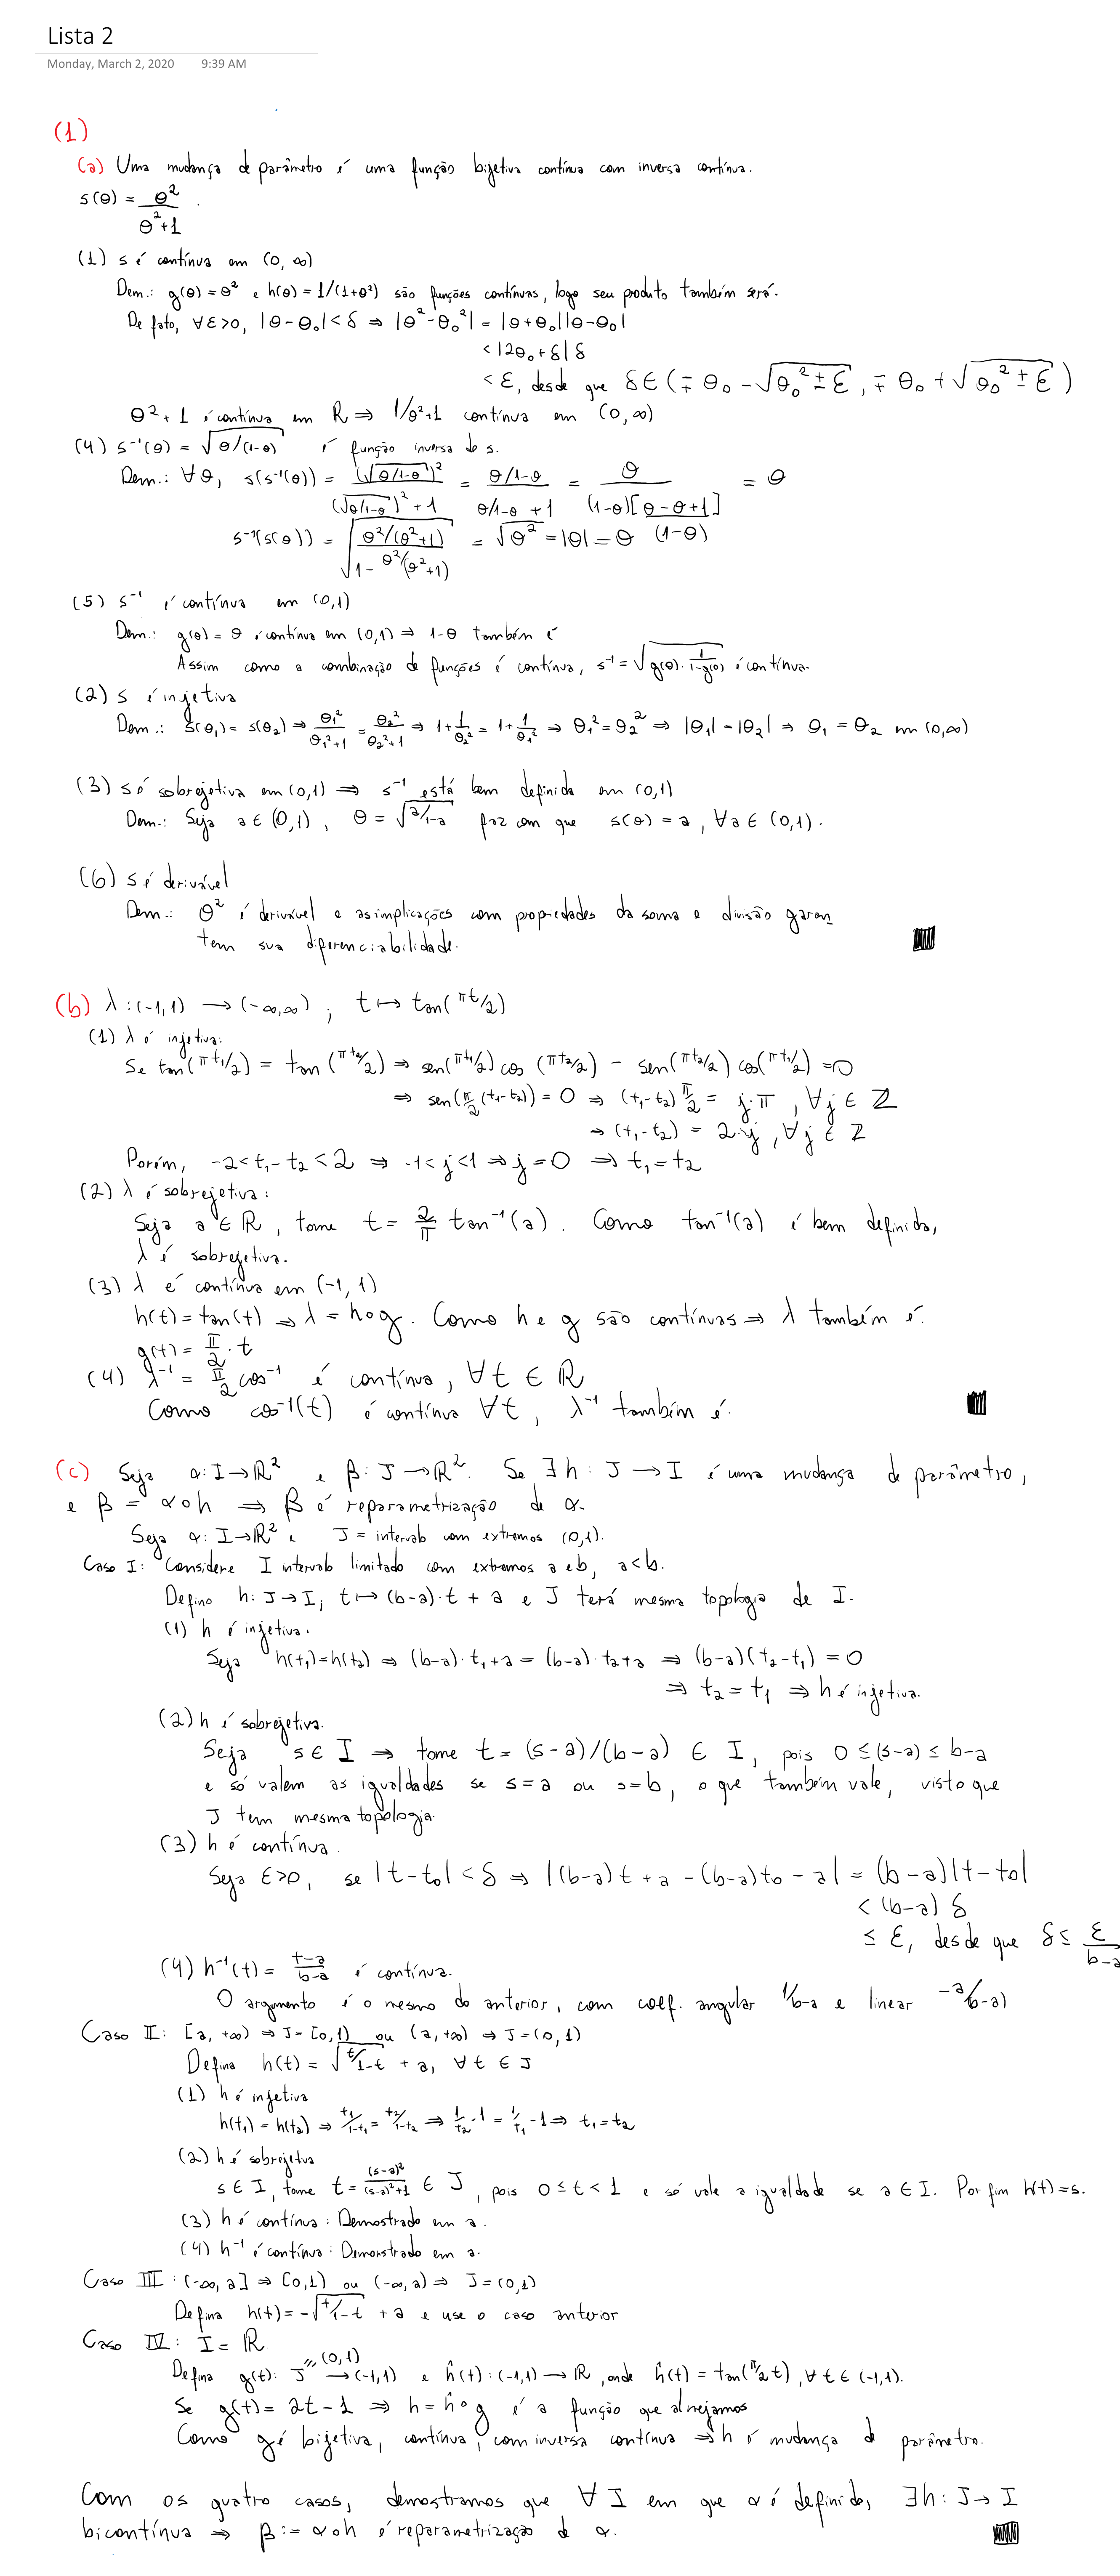
\includegraphics[width = \textwidth,trim=1.5in 24in 1in 3.6in, clip]{images/exe4.png}
    \end{figure}
    \clearpage
    \begin{center}
        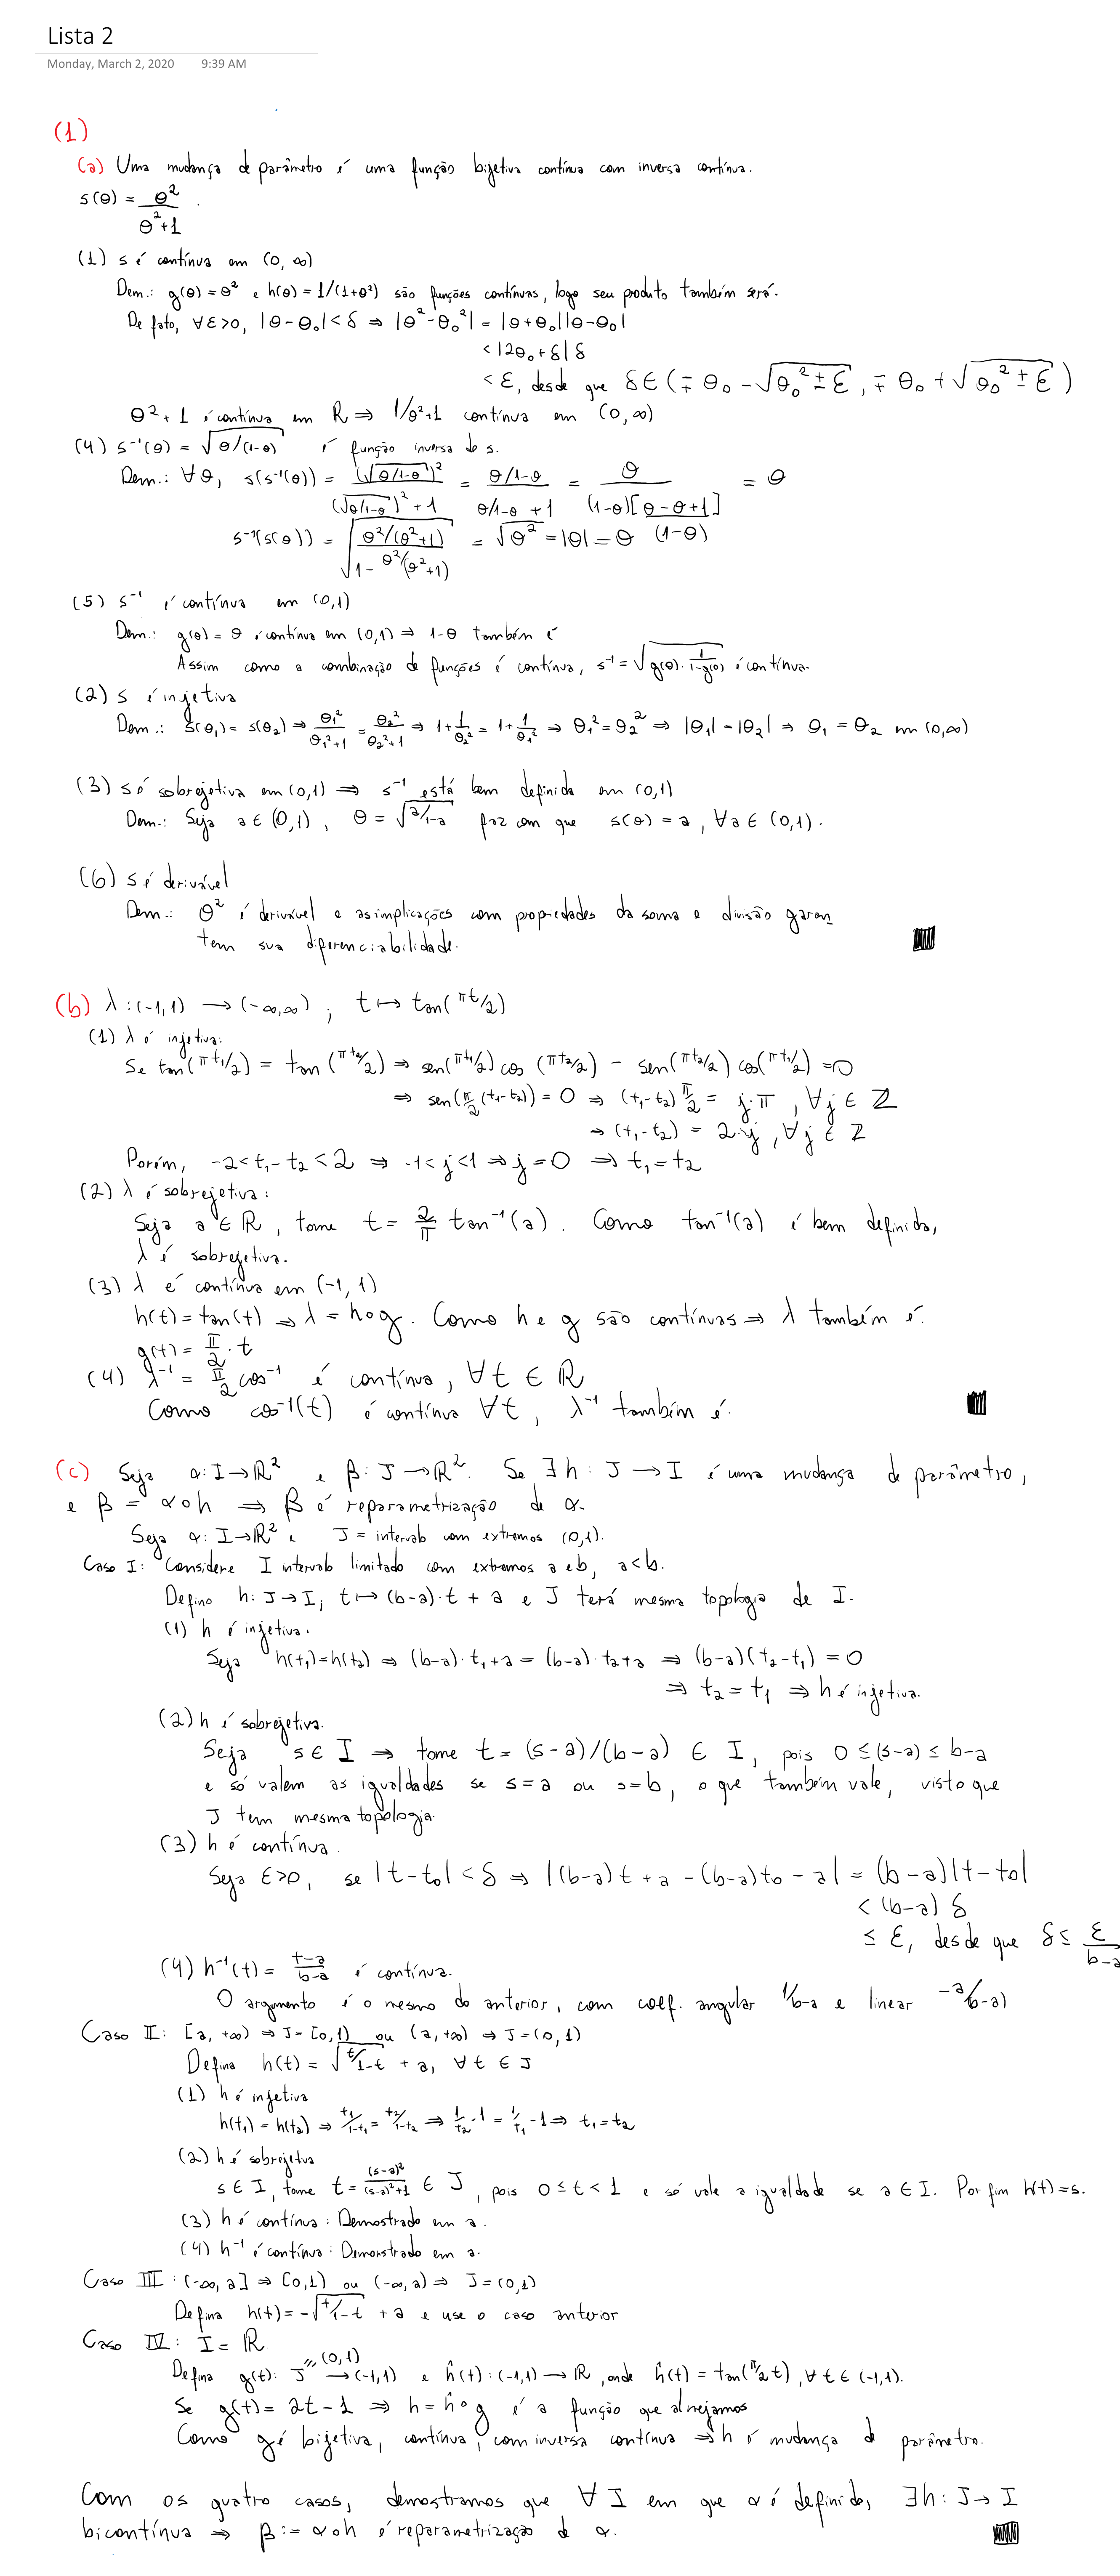
\includegraphics[width=\textwidth, trim=1.5in 0in 0in 40in, clip]{images/exe4.png}
    \end{center}
    
\end{solution}

\begin{exercise}
    Provar que a curva
    $$\gamma(t) = \left(2t, \frac{2}{1+t^2}\right)$$ 
    com $t > 0$ é regular e é uma reparametrização de
    $$\alpha(t) = \left(\frac{2\cos(t)}{1 + \sin(t)}, 1 + \sin(t)\right), t
    \in (-\pi/2, \pi/2)$$
\end{exercise}

\begin{solution}
    Para provar que a curva é regular, basta observar que 
    $$
    \gamma '(t) = \left(2, -4\frac{t}{(1+ t^2)^2}\right) \neq (0,0), \forall t > 0
    $$
    Para verificar que $\alpha$ é uma reparametrização, devemos achar uma
    mudança de parâmetro $h$ tal que $\alpha = \gamma \circ h$. Em particular,
    queremos que a primeira coordenada seja igual
    $$
    \frac{2\cos(t)}{1 + \sin(t)} = 2h(t) \implies h(t) = \frac{\cos(t)}{1 + \sin(t)}
    $$
    tanto quanto a segunda 
    $$
    1 + \sin(t) = \frac{2}{1 + h(t)^2} = \frac{2}{1 + \frac{\cos(t)^2}{(1 + \sin(t))^2}} = \frac{2(1 + \sin(t))^2}{1 + 2\sin(t) + \sin(t)^2 + \cos(t)^2} = 1 + \sin(t)
    $$
    portanto sugerimos a função $h$ acima definida com domínio
    $(-\pi/2,\pi/2)$ e contradomínio $(0, + \infty)$. É fácil que $h$ é
    contínua (combinação de funções contínuas) e derivável (combinação de
    funções deriváveis). Vamos verificar a bijetividade: 
    \begin{enumerate}
        \item (Injetividade) Afirmo que $h$ é estritamente decrescente no
        intervalo especificado: 
        $$
        h'(t) = \frac{-\sin(t) -\sin^2(t) - \cos^2(t)}{(1 + \sin(t))^2} = -\frac{1}{1 + \sin(t)} < 0, 
        $$
        pois $|\sin(t)| < 1$ entre $(-\pi/2, \pi/2)$. Logo a função é
        estritamente decrescente e, por consequência, injetiva. 
        
        \item (Sobrejetividade) Tome $x > 0$. Vamos encontrar a inversa $g$ de
        $h$. Se ela existir, ela terá a forma: 
        $$
        h(g(x)) = x \implies \frac{\cos(g(x))}{1 + \sin(g(x))} = x \implies \frac{\cos^2(g(x))}{(1 + \sin(g(x)))^2} + 1 = x^2 + 1
        $$
        Portanto, fazendo a soma de frações, obtemos
        $$
        1 + x^2 = \frac{2}{1 + \sin(g(x))} \implies g(x) = \sin^{-1}\left(\frac{1 - x^2}{1 + x^2}\right)
        $$
        Quando $x \in (0,1)$, a expressão entre parênteses está entre $(0,1)$
        também (só invertendo os limites) e portanto $g(x) \in (0, \pi/2)$.
        Mas quando $x \ge 1$, a expressão entre parênteses está entre $(-1,
        0]$ e, portanto $g(x) \in (-\pi/2, 0]$. Assim o contradomínio de $g$ é
        $(-\pi/2, \pi/2)$ o que mostra que $h$ é sobrejetiva. Além disso,
        observe que $g(h(t)) = t$ (verifique as contas) e $h(g(x)) = x$ o que
        mostra que $g$ é a inversa de $h$. 
    \end{enumerate}
    Precisamos mostrar que $g$ é contínua e derivável. Mas ela é em seu
    domínio $(0, +\infty)$, pois é combinação de funções contínuas e
    deriváveis. 
    Em particular $\gamma$ e $\alpha$ são reparametrizações. 
\end{solution}

\begin{exercise}
    Seja $\alpha(t) = \left(\frac{1}{\sqrt{3}}\cos(t) + \frac{1}{\sqrt{2}}\sin(t),
    \frac{1}{\sqrt{3}}\cos(t), \frac{1}{\sqrt{3}}\cos(t) -
    \frac{1}{\sqrt{2}}\sin(t)\right)$. Reparametrizar $\alpha$ pelo
    comprimento de arco.
\end{exercise}

\begin{solution}
    Nesse exercício, queremos que encontrar uma reparametrização de $\alpha$
    que tenha velocidade unitária. Para isso existir $\alpha$ deve ser
    regular. Vamos calcular $\alpha '(t)$: 
    $$ 
    \alpha '(t) = -\left(\frac{1}{\sqrt{3}}\sin(t) - \frac{1}{\sqrt{2}}\cos(t), \frac{1}{\sqrt{3}}\sin(t), \frac{1}{\sqrt{3}}\sin(t) + \frac{1}{\sqrt{2}}\cos(t)\right)
    $$
    Observe que 
    \begin{multline}
        ||\alpha '(t)||^2 = \frac{1}{3}\sin^2(t) - \frac{2}{\sqrt{6}}\sin(t)\cos(t) + \frac{1}{2}\cos^2(t) + \frac{1}{3}\sin^2(t) \\ + \frac{1}{3}\sin^2(t) + \frac{2}{\sqrt{6}}\sin(t)\cos(t) + \frac{1}{2}\cos^2(t) = \sin^2(t) + \cos^2(t) = 1
    \end{multline}
    Portanto $\alpha$ já está parametrizada pelo comprimento de arco. 
\end{solution}

\begin{exercise}
    Mostre que, se todas as retas tangentes a uma curva regular passam por um
    mesmo ponto $P \in \R^2$, então seu traço está contido em uma reta.
\end{exercise}

\begin{solution}
    Seja $\gamma$ uma regular e suponha, sem perda de generalidade (s. p. g.)
    que ela esteja parametrizada pelo comprimento de arco. Defina $t(s ) =
    \dot{\gamma}(s)$. Para cada $s$,
    existe $\beta(s)$ tal que $\beta(s)t(s) + \gamma(s) = P$, isto
    é, a reta que passa pelo ponto $\gamma(s)$ tangente à curva, passa pelo
    ponto $P$ com coeficiente $\beta(s)$. Em particular, podemos definir 
    $\beta(s)$ como 
    $$
    \beta(s)t(s)\cdot t(s) = (P - \gamma(s))\cdot t(s) \implies \beta(s) = (P - \gamma(s))t(s),
    $$
    dado que $t(s)\cdot t(s) = 1$. Estamos supondo $\gamma$ uma curva de
    classe pelo menos $C^2$. Portanto $\beta$ é diferenciável e 
    $$
    0 = \frac{d}{ds}(\beta(s)t(s) + \gamma(s)) = \dot{\beta}(s)t(s) + \beta(s)\dot{t}(s) + t(s)
    $$
    Onde a derivada é nula, pois a expressão vale $P$ para todo $s$.
    Sabemos que $\langle t, \dot{t} \rangle = 0$ como provamos na lista 1.
    Assim, se aplicarmos o produto interno com $\dot{t}$ em ambos os lados,
    teremos 
    $$
    0 = \beta(s)||\dot{t}(s)||^2
    $$
    Portanto, para todo $s$, temos que $\beta(s) = 0$ ou $\dot{t}(s) = 0$.
    Suponha que $\dot{t}(s) \neq 0$ para algum $s$. Então pela continuidade
    de $\dot{t} = \ddot{\gamma}$, teremos que existe um intervalo aberto em
    torno de $s$ que $\dot{t}$ é não nulo nesse intervalo. Entretanto
    $\beta(s)$ deve ser 0 nesse intervalo e portanto $\gamma(s) = P$ nesse
    intervalo. Mas se $\gamma$ é constante nesse intervalo, teremos que
    $\dot{\gamma} = 0$ nesse intervalo, o que é uma contradição. Concluímos
    que $\ddot(\gamma) = 0 \implies \dot{\gamma} = constante$ e, portanto,
    o traço de $\gamma$ está contido em uma reta\footnote{\url{https://lucasmoschen.github.io/ta-sessions/curvas/first-definitions/\#proposicao}}. 
\end{solution}

\begin{exercise}
    Mostre que, se todas as retas normais a uma curva regular passam por um
    mesmo ponto $P \in \R^2$, então seu traço está contido em um círculo.
\end{exercise}

\begin{solution}
    Seja $\gamma$ uma curva regular parametrizada pelo comprimento de arco,
    sem perda de generalidade. Em cada ponto $\gamma(s)$ passa uma reta
    com direção $\gamma ''(s)$ que passa por $P$. Em particular, todas as
    retas tem o formato 
    $$
    P + \alpha\gamma ''(s), \alpha \in \R
    $$
    Para cada $s$ existe $\alpha_s$ tal que 
    $$
    P + \alpha_s\gamma ''(s) = \gamma(s) \implies \alpha_s\gamma ''(s) = \gamma(s) - P
    $$
    Produto interno com $\gamma '(s)$ faz com que $\langle \gamma(s) - P, \gamma '(s) \rangle = 0$.
    Em particular 
    $$
    \frac{d}{ds}||\gamma(s) - P||^2 = \langle \gamma '(s), \gamma(s) - P \rangle + \langle \gamma(s) - P, \gamma '(s) \rangle = 0 
    $$
    o que mostra que $||\gamma(s) - P||$ é constante, o que caracteriza (parte
    de) uma circunferência.
\end{solution}

\end{document}